\documentclass[xcolor=dvipsnames,10pt]{beamer}

\mode<presentation> {
    \usetheme{Madrid}
    \setbeamertemplate{theorems}[numbered]
    \usecolortheme[RGB={115,0,60}]{structure}
}

\usepackage{amsmath}
\usepackage{amsfonts,amssymb,amsthm,bbm,enumerate,graphicx,color,mathtools}
\usepackage[spanish]{babel}
\usepackage[utf8]{inputenc}

\usepackage{mathpazo}
\usepackage{pgf,tikz}
\usetikzlibrary{arrows}
\usepackage{epic,eepic}
\usepackage{hyperref}


\newcommand{\abs}[1]{\left\vert#1\right\vert}
\newcommand{\set}[1]{\left\{#1\right\}}
\newcommand{\R}{\mathbb{R}}
\newcommand{\Z}{\mathbb{Z}}
\newcommand{\N}{\mathbb{N}}
\newcommand{\T}{\mathbb{T}}
\renewcommand{\a}{\alpha}
\renewcommand{\b}{\beta}
\newcommand{\s}{\sigma}
\renewcommand{\t}{\theta}
\renewcommand{\v}{\varphi}
\renewcommand{\L}{\mathcal{L}}
\renewcommand{\P}{\mathcal{P}}
\newcommand{\J}{\mathcal{J}}
\newcommand{\K}{\mathcal{K}}
\newcommand{\blue}[1]{\textcolor{blue}{#1}}
\newcommand{\red}[1]{\textcolor{red}{#1}}
\newcommand{\rioja}[1]{\textcolor[RGB]{115,0,60}{#1}}
\newcommand{\PV}{\operatorname{P.V.}}
\newcommand{\x}{\mathtt{x}}
\DeclareMathOperator*{\essup}{ess\,sup}
\DeclareMathOperator*{\loc}{loc}
\DeclareMathOperator*{\supesn}{sup\,esn}

\renewcommand{\Re}{\operatorname{Re}}
\renewcommand{\Im}{\operatorname{Im}}
\renewcommand{\lim}{\operatorname{lim}}
\renewcommand{\S}{\mathbb{S}}
\renewcommand{\div}{\operatorname{div}}
\newcommand{\Id}{\operatorname{Id}}
\newcommand{\RP}{\mathbb{RP}}
\newcommand{\CP}{P_\ell(\mathbb{C})}
\newcommand{\HP}{P_\ell(\mathbb{H})}
\newcommand{\Ca}{P_2(\mathbb{C}\mathbbm{a}\mathbbm{y})}
\newcommand{\B}{\mathbb{B}}
\newcommand{\supp}{supp}
\newcommand{\mb}[1]{\mathbf{#1}}

\newtheorem*{thm}{Teorema}
\newtheorem*{app}{Aplicación}
\newtheorem{thma}{Teorema}
\newtheorem*{MTheo}{Teorema Principal}
\newtheorem*{Def}{Definición}
\newtheorem*{Prop}{Proposición}
\newtheorem{Propo}{Proposición}
\newtheorem*{Lem}{Lema}
\newtheorem*{Cor}{Corolario}
\newtheorem*{Mcor}{Corolario Principal}
\newtheorem{rem*}{Comentario}

% --- DATOS DEL TFG ---
\title 
[La función hipergeométrica de Gauss] 
{{\huge La función hipergeométrica de Gauss}}

\subtitle{Gauss's hypergeometric function}

\author[D. González]{%
    \texorpdfstring{{\Large Daniel González Espinosa} \\ \vspace{0.4cm} \normalsize Dirigido por: Óscar Ciaurri Ramírez}{Daniel González Espinosa}%
}

\institute[UR]
{Grado en Matemáticas\\
Universidad de La Rioja}

\date[Junio 2026] 
{Logroño, Junio de 2026}

\subject{La función hipergeométrica de Gauss}

\titlegraphic{
\includegraphics[height=2.2cm]{logo_unirioja.png}}

\begin{document}

\begin{frame}[plain]
  \titlepage
\end{frame}

\section{Introducción}

\begin{frame}{Introducción}
    \begin{columns}
        \begin{column}{0.4\textwidth}
            \centering
            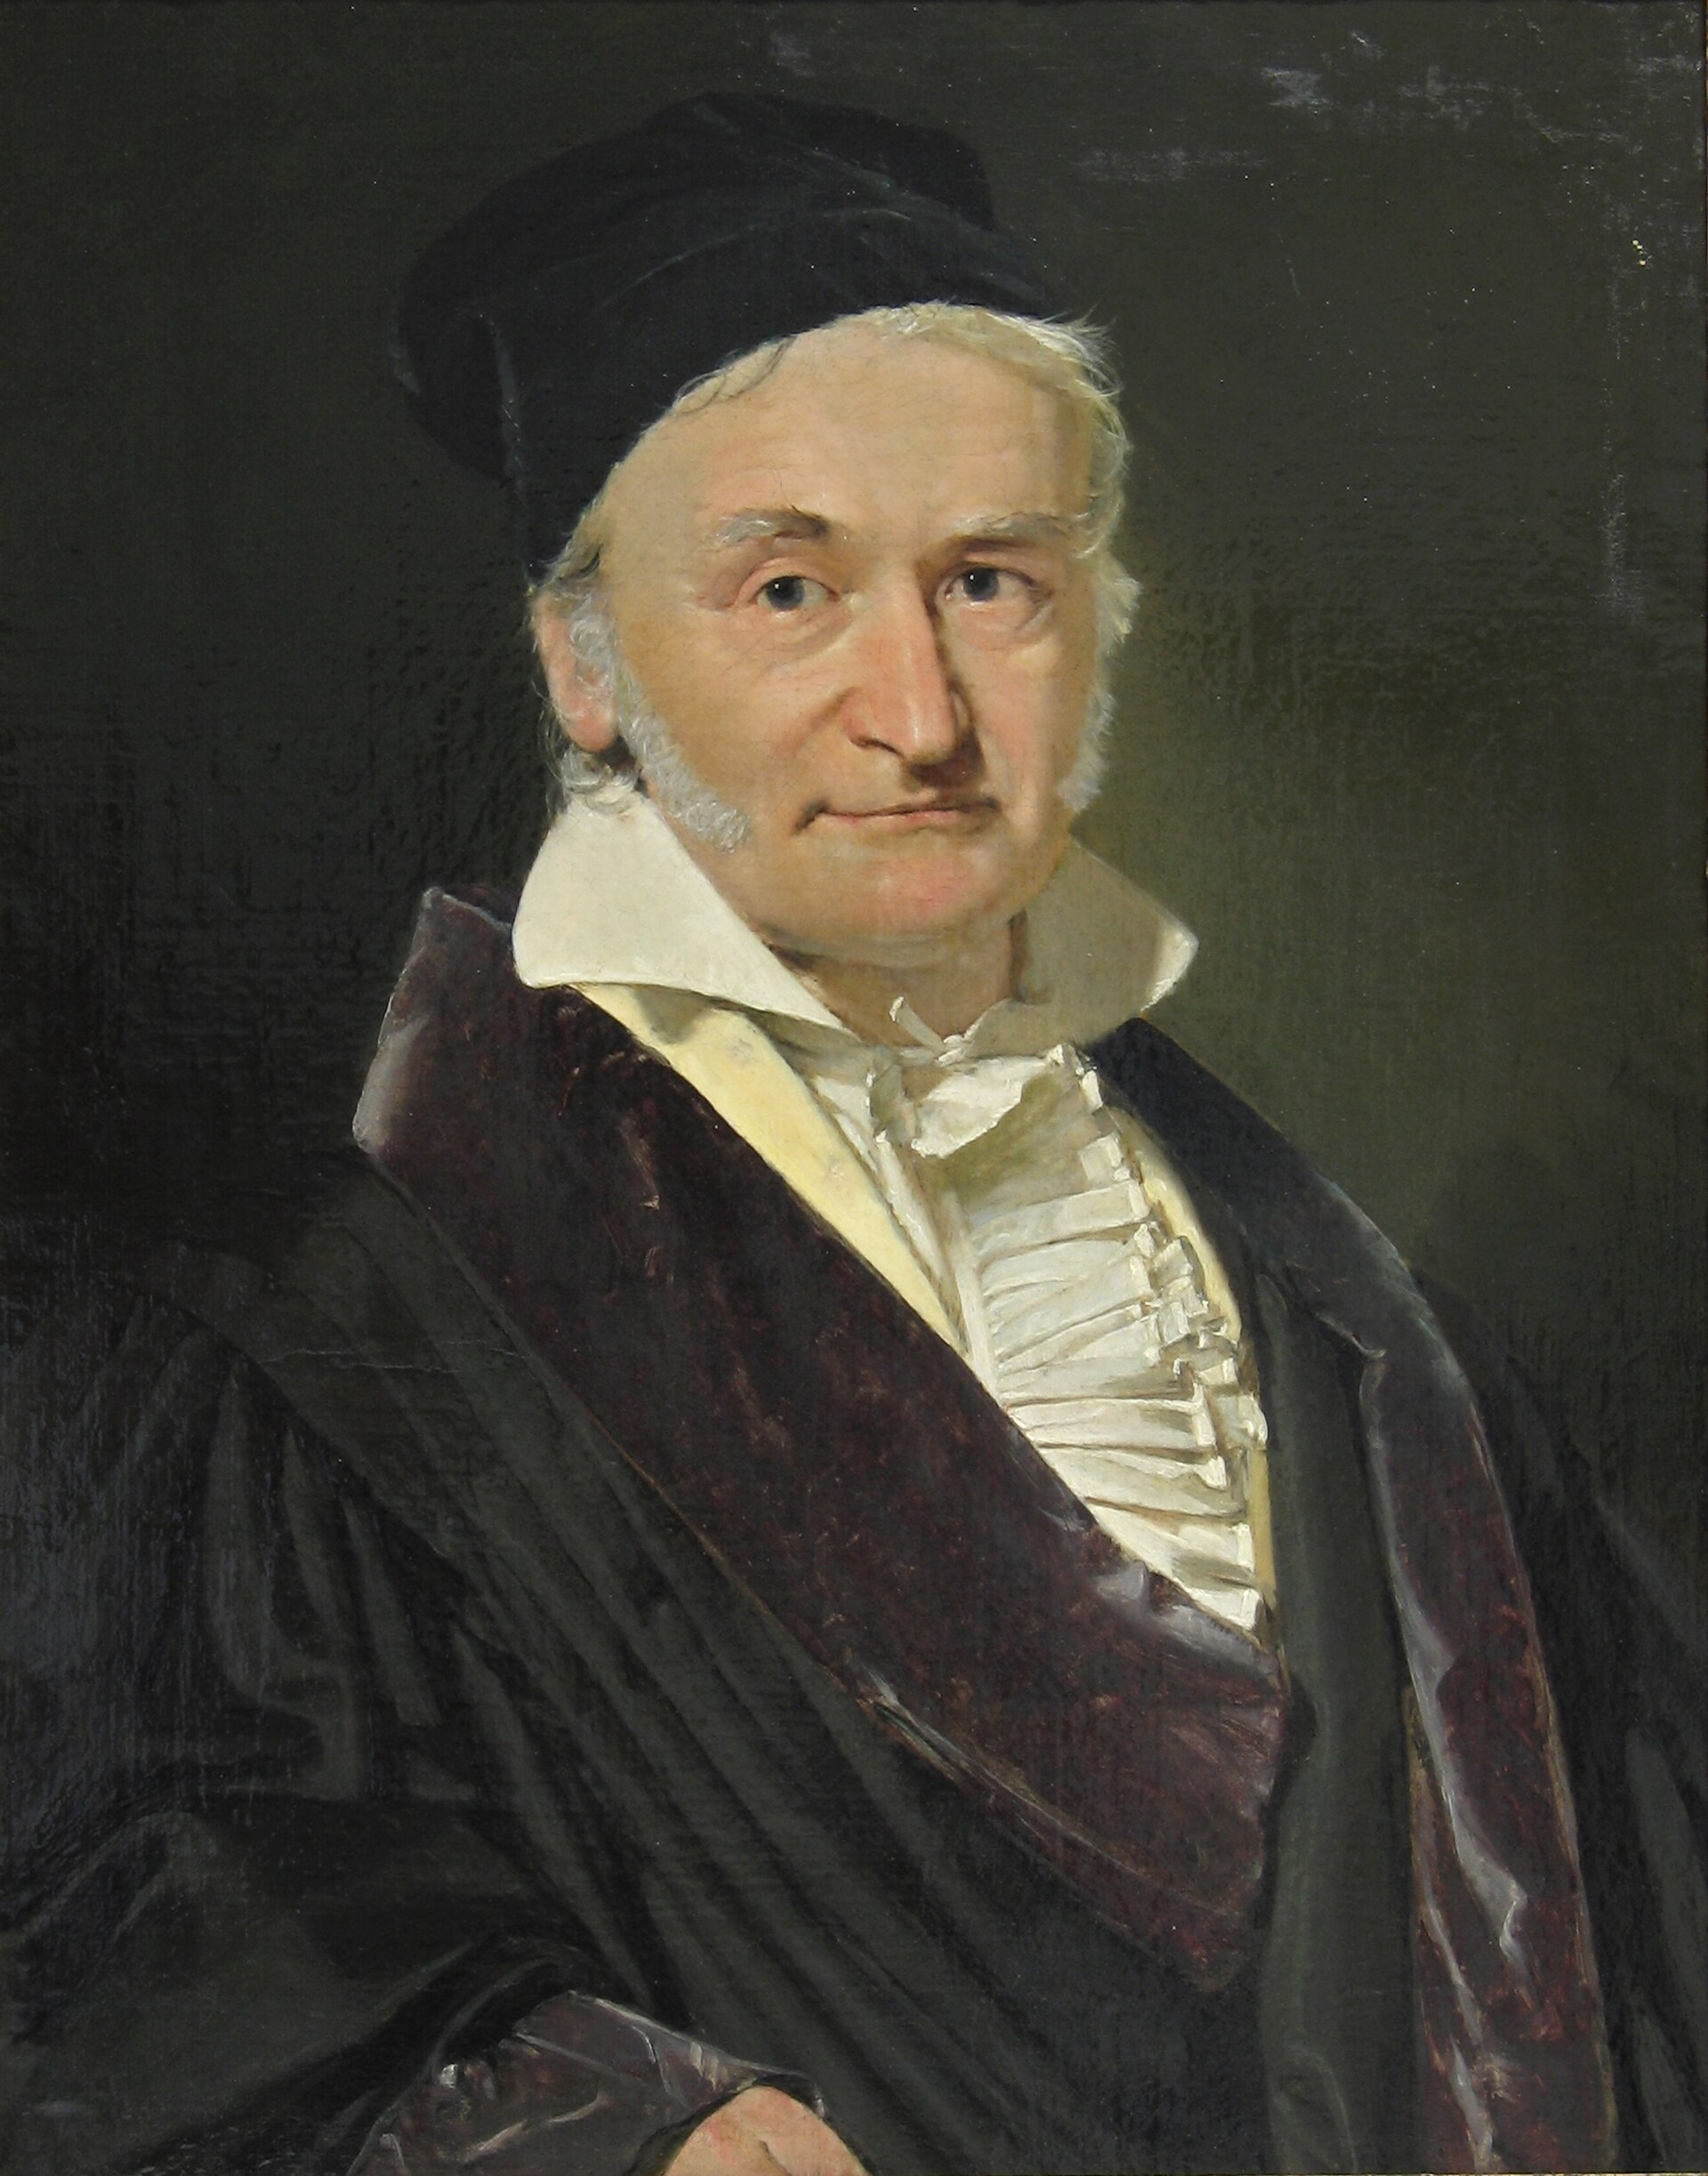
\includegraphics[width=\linewidth]{gauss.jpg}\\
            \vspace{-0.1cm}
            {\small Carl Friedrich Gauss (1777--1855)}
        \end{column}

        \begin{column}{0.6\textwidth}
            La función hipergeométrica de Gauss constituye uno de los objetos analíticos más versátiles de la teoría de funciones especiales. Su principal valor radica en su capacidad como marco unificador, permitiendo englobar una vasta gama de funciones elementales y trascendentes mediante la elección de sus parámetros.

            \vspace{0.2cm}
            \visible<2->{
            El primer tratamiento sistemático lo dió Gauss en 1812.
            }
           

            \vspace{0.2cm}
            \visible<3->{Este trabajo se estructura en tres ejes fundamentales:}
            \begin{itemize}
                \item<3-> Definición y primeras propiedades.
                \item<4-> Conexión con los polinomios ortogonales.
                \item<5-> Desarrollo de identidades hipergeométricas.
            \end{itemize}
        \end{column}
    \end{columns}
\end{frame}

\section{Definición y primeras propiedades}
\subsection{Definición}

\begin{frame}{Definición de la función hipergeométrica}
    Dados tres parámetros complejos $a, b, c \in \mathbb{C}$ y una variable compleja $z$, la \rioja{función hipergeométrica de Gauss} se define a través de la serie de potencias
    \[
    {}_{2}F_{1}(a,b;c;z) = \sum_{n=0}^{\infty} \frac{(a)_{n}(b)_{n}}{(c)_{n}} \frac{z^{n}}{n!},
    \]
    \vspace{-0.2cm}
    donde $(x)_{n}$ es el \rioja{símbolo de Pochhammer} definido como
    \[
    (x)_{n} = \begin{cases} 1, & \text{si } n=0, \\ x(x+1)\cdots(x+n-1), & \text{si } n>0. \end{cases}
    \]
    
    \vspace{-0.2cm}
    \visible<2->{
    El \rioja{símbolo de Pochhammer} también puede expresarse para todo $x \neq 0, -1, -2, \dots$ como
    \vspace{-0.2cm}
    \[
    (x)_{n} = \frac{\Gamma(x+n)}{\Gamma(x)}.
    \]
    }

    \vspace{-0.2cm}
    \visible<3->{
    Los parámetros $a$ y $b$ pueden ser números complejos cualesquiera y la función es simétrica con respecto a ellos.
    \vspace{-0.2cm}
    \[
    {}_{2}F_{1}(a,b;c;z) = {}_{2}F_{1}(b,a;c;z).
    \]
    }
\end{frame}

\begin{frame}{Condiciones sobre los parámetros y ejemplos}
    Por otro lado, cuando el parámetro $a=-m$ es un entero no positivo, la serie se trunca, dando lugar a un polinomio de grado $m$ en $z$.

    \visible<2->{
    El parámetro $c$ debe cumplir que $c \neq 0, -1, -2, \dots$. Para evitar esta restricción, utilizamos la versión regularizada
    \[
    {}_{2}\tilde{F}_{1}(a,b;c;z) = \frac{{}_{2}F_{1}(a,b;c;z)}{\Gamma(c)} = \sum_{n=0}^{\infty} \frac{(a)_{n}(b)_{n}}{\Gamma(c+n)} \frac{z^{n}}{n!}.
    \]
    }
    
    \vspace{-0.2cm}
    \visible<3->{
    Estas propiedades consolidan a la serie como un auténtico marco unificador de funciones elementales.
    \[
    \begin{aligned}
        {}_{2}F_{1}(1,b;b;z) &= \frac{1}{1-z}, & {}_{2}F_{1}(-a,b;b;-z) &= (1+z)^{a}, \\
        z \cdot {}_{2}F_{1}(1,1;2;-z) &= \log(1+z), & z \cdot {}_{2}F_{1}(\tfrac{1}{2},\tfrac{1}{2};\tfrac{3}{2};z^2) &= \text{arcsen } z,
    \end{aligned}
    \]
    permitiendo incluso representar la integral elíptica completa de primera especie
    \[
    \frac{\pi}{2} \cdot {}_{2}F_{1}\left(\frac{1}{2}, \frac{1}{2}; 1; k^2\right)= \int_{0}^{\pi/2} \frac{d\theta}{\sqrt{1-k^2 \sin^{2}{\theta}}} = K(k), \quad \text{con } 0 \leq k <1.
    \]}
\end{frame}

\subsection{Convergencia de la serie hipergeométrica}

\begin{frame}{Convergencia en el disco unidad y resultados previos}

    El dominio de validez de la serie hipergeométrica se establece de manera directa analizando el límite del valor absoluto del cociente de dos términos consecutivos
    \[
    L = \lim_{n\to\infty} \left| \frac{T_{n+1}}{T_n} \right| = \lim_{n\to\infty} \left| \frac{(a+n)(b+n)}{(c+n)(n+1)} z \right| = |z|.
    \]
    
    \vspace{-0.1cm}
    \visible<2->{
    De este modo, el criterio del cociente garantiza que la serie converge absolutamente para $|z|<1$ y diverge para $|z|>1$, fijando un radio de convergencia $R=1$. El análisis en la frontera exige ser más preciso.
    }

    \vspace{0.1cm}
    \visible<3->{
    A tal efecto, se demuestra un lema sobre el cociente de funciones Gamma. Para $p, q \in \mathbb{C}$ fijos
    \vspace{-0.1cm}
    \[
    \frac{\Gamma(n+q)}{\Gamma(n+p)} \sim n^{q-p}\left(1+\frac{(q-p)(q+p-1)}{2n}\right).
    \]
    }
    
    \vspace{-0.1cm}
    \visible<4->{
    Al aplicar esta aproximación sobre el término general $T_n = u_n z^n$, se obtiene la descomposición asintótica
    \begin{equation}
        \label{eq:asintotica_tn}
        T_n \sim C_1 n^{a+b-c-1} z^n + C_2 n^{a+b-c-2} z^n.
    \end{equation}
    }
\end{frame}

\begin{frame}{Convergencia en la frontera}
    \begin{block}{Teorema}
        Sea $\delta = \Re(c-a-b)$. En la circunferencia unidad $|z|=1$, la serie hipergeométrica ${}_{2}F_{1}(a,b;c;z)$,
        \begin{enumerate}
            \item converge absolutamente si $\delta > 0$,
            \item converge condicionalmente si $-1 < \delta \le 0$, siempre que $z \neq 1$, y
            \item diverge si $\delta \le -1$.
        \end{enumerate}
        La serie también diverge en $z=1$ si $\delta \leq 0$.
    \end{block}
    
    \vspace{0.1cm}
    \begin{overprint}
        \onslide<2>
        En el caso $\delta > 0$, por \eqref{eq:asintotica_tn} tenemos que 
        \[
        \sum_{n=1}^\infty |T_n| \le C\sum_{n=1}^\infty n^{-\delta -1},
        \]
        que es convergente por ser $\delta > 0$.

        \onslide<3>
        Cuando $-1 < \delta \le 0$ y $z = e^{i\theta} \neq 1$, utilizamos el \rioja{criterio de Dirichlet}. Las sumas parciales de la componente oscilatoria $e^{in\theta}$ permanecen acotadas, mientras que la parte real decrece monótonamente hacia cero.

        \onslide<4>
        Finalmente, si $\delta \le -1$, de \eqref{eq:asintotica_tn} deducimos que $\lim_{n\to\infty} \abs{T_n} \neq 0$. 
        Además, si $z=1$ y $-1 < \delta \le 0$ tenemos que 
        \[
        \sum_{n=1}^\infty T_n \sim C_1 \sum_{n=1}^\infty n^{-(c-a-b)-1} + C_2 \sum_{n=1}^\infty n^{-(c-a-b)-2}.
        \]
        La segunda de estas series es convergente pero la primera es divergente por ser $-1 < \delta \le 0$.
    \end{overprint}
\end{frame}

\subsection{La representación integral y la extensión analítica}

\begin{frame}{Representación integral y extensión analítica}

    Como hemos comprobado, la serie hipergeométrica diverge fuera del disco unidad. Para sortear esta limitación y extender su dominio, recurrimos a la \rioja{representación integral de Euler}.

    \visible<2->{
    \begin{block}{Teorema}
        Para $\Re(c) > \Re(b) > 0$ y $|z| < 1$, se verifica
        \[
        {}_{2}F_{1}(a, b; c; z) = \frac{\Gamma(c)}{\Gamma(b)\Gamma(c-b)} \int_{0}^{1} t^{b-1}(1-t)^{c-b-1}(1-zt)^{-a} \, dt.
        \]
    \end{block}
    }

    \vspace{0.1cm}
    \begin{columns}[T] 
        \begin{column}{0.6\textwidth}
            \visible<3->{
            El integrando desvela que esta expresión no solo recupera la serie original, sino que define una función analítica en el plano complejo  $D_I = \mathbb{C} \setminus [1, \infty)$.
            }
            
            \vspace{0.3cm}
            \visible<5->{
            Aplicando el \rioja{principio de prolongación analítica}, garantizamos que esta extensión desde el disco a todo el dominio $D_I$ es única.
            }
        \end{column}
        
        \begin{column}{0.35\textwidth}
            \centering
            \vspace{-0.3cm}
            \visible<4->{
            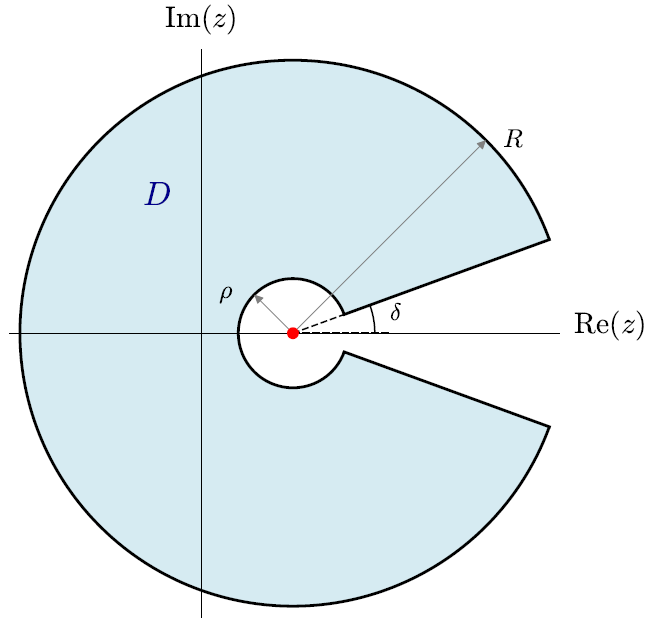
\includegraphics[width=3.85cm]{dominio_D.png}
            }
        \end{column}
    \end{columns}
\end{frame}

\begin{frame}{Teorema de Gauss y Chu-Vandermonde}

    Aunque la integral de Euler restringe los parámetros a $\Re(c) > \Re(b) > 0$, el uso iterativo de relaciones de recurrencia permite extender analíticamente la función para todo $a$, $b \in \mathbb{C}$ y $c \in \mathbb{C} \setminus \{0,-1,-2,\dots\}$.

    \visible<2->{
    \begin{block}{Teorema}
        Si se cumple la condición $\Re(c - a - b) > 0$, entonces
        \[
        {}_{2}F_{1}(a, b; c; 1) = \frac{\Gamma(c)\Gamma(c - a - b)}{\Gamma(c - a)\Gamma(c - b)}.
        \]
    \end{block}
    }

    \visible<3->{Como consecuencia directa, cuando la serie se trunca al tomar $a = -n$, aparece la \rioja{identidad de Chu-Vandermonde}
    \vspace{-0.2cm}
    \[
    {}_{2}F_{1}(-n, b; c; 1) = \frac{(c-b)_n}{(c)_n}.
    \]
    }

    \vspace{-0.3cm}
    \visible<4->{Esta identidad es  equivalente a la identidad combinatoria de Vandermonde.}

\end{frame}

\subsection{Transformaciones lineales}

\begin{frame}{Transformaciones lineales}

    La estructura analítica de la función hipergeométrica permite establecer identidades fundamentales para modificar sus parámetros.
    
    \vspace{0.1cm}
    \visible<2->{
    Un primer resultado viene dado por la \rioja{transformación de Pfaff}, válida para $|\arg(1-z)|<\pi$,
    \[
    {}_{2}F_{1}(a, b; c; z) = (1-z)^{-a} {}_{2}F_{1}\left(a, c-b; c; \frac{z}{z-1}\right).
    \]    
    }
    
    \visible<3->{
    Este vínculo se deduce a partir de la representación integral de Euler y aunque la integral exige que $\Re(c) > \Re(b) > 0$, el \rioja{principio de prolongación analítica} garantiza la validez de la identidad en todo su espacio de parámetros.
    }
    
    \vspace{0.2cm}
    \visible<4->{
    Si aplicamos de nuevo la transformación de Pfaff aparece la \rioja{transformación de Euler}, también válida para $|\arg(1-z)|<\pi$,
    \[
    {}_{2}F_{1}(a, b; c; z) = (1-z)^{c-a-b} {}_{2}F_{1}(c-a, c-b; c; z).
    \]
    }
\end{frame}

\subsection{Identidades en valores especiales}

\begin{frame}{Identidades en valores especiales}

    La representación integral también nos sirve para hallar el valor de la función en puntos específicos del plano complejo bajo ciertas condiciones, destacamos el \rioja{teorema de Kummer} en $z=-1$, 
    \vspace{-0.3cm}
    \[
    {}_{2}F_{1}(a, b; 1-a+b; -1) = \frac{\Gamma(1-a+b) \Gamma(1+\frac{b}{2})}{\Gamma(1+\frac{b}{2}-a) \Gamma(1+b)},
    \]

    \vspace{-0.1cm}
    \visible<2->{
    la \rioja{identidad de Bailey} en $z=1/2$, 
    \vspace{-0.3cm}
    \[
    {}_{2}F_{1}(a, 1-a; c; \tfrac{1}{2}) = \frac{\Gamma(\frac{c}{2})\Gamma(\frac{c+1}{2})}{\Gamma(\frac{c+a}{2})\Gamma(\frac{c-a+1}{2})},
    \]
    }

    \vspace{-0.1cm}
    \visible<3->{
    el \rioja{segundo teorema de Gauss} en $z=1/2$,
    \vspace{-0.3cm}
    \[
    {}_{2}F_{1}(a, b; \tfrac{a+b+1}{2}; \tfrac{1}{2}) = \frac{\sqrt{\pi} \Gamma(\frac{a+b+1}{2})}{\Gamma(\frac{a+1}{2})\Gamma(\frac{b+1}{2})},
    \]
    }
    
    \vspace{-0.1cm}
    \visible<4->{
    y la \rioja{fórmula de Gosper} en $z=1/4$,
    \vspace{-0.3cm}
    \[
    {}_{2}F_{1}\left(\tfrac{1}{2}, b; \tfrac{5}{2}-2b; \tfrac{1}{4}\right) = \frac{2^{2b}\sqrt{\pi}}{3}\frac{\Gamma(\frac{5}{2}-2b)}{\Gamma^{2}(\frac{3}{2}-b)}.
    \]
    }
\end{frame}

\section{Conexión con polinomios ortogonales}

\subsection{Polinomios de Jacobi}

\begin{frame}{Polinomios de Jacobi}

    Para parámetros $\alpha, \beta > -1$, el \rioja{polinomio de Jacobi} de grado $n$, $P_n^{(\alpha, \beta)}(x)$ se define mediante la \rioja{fórmula de Rodrigues}
    \[
    P_n^{(\alpha, \beta)}(x) = \frac{(-1)^n}{2^n n!} (1-x)^{-\alpha} (1+x)^{-\beta} \frac{d^n}{dx^n} \left( (1-x)^{\alpha+n} (1+x)^{\beta+n} \right).
    \]

    \vspace{-0.1cm}
    \visible<2->{
    Aplicando la regla de Leibniz para la derivada de un producto sobre esta expresión, se demuestra que todos los factores se cancelan adecuadamente, garantizando que $P_n^{(\alpha, \beta)}(x)$ constituye un polinomio de grado exactamente $n$.
    }

    \visible<3->{
    El desarrollo de esta derivada permite evaluar  el polinomio y su primera derivada en el punto $x=1$, verificando que
    \[
     P_n^{(\alpha, \beta)}(1) = \binom{n+\alpha}{n} \quad \text{y} \quad (P_n^{(\alpha, \beta)})'(1) = \frac{n+\alpha+\beta+1}{2} \binom{n+\alpha}{n-1}.
    \]
    
    \vspace{-0.2cm}
    Estos valores exactos resultarán indispensables para establecer la identidad definitiva que vincula esta familia polinómica con la función hipergeométrica.
    }
\end{frame}

\begin{frame}{Ecuación diferencial de Jacobi}

    Una de las propiedades fundamentales de los polinomios de Jacobi es que son soluciones de una ecuación diferencial lineal de segundo orden.

    \vspace{0.1cm}
    \visible<2->{
    \begin{block}{Teorema}
        El polinomio $y(x) = P_n^{(\alpha, \beta)}(x)$ satisface la siguiente ecuación diferencial homogénea de segundo orden
        \[
        (1-x^2)y'' + (\beta - \alpha - (\alpha + \beta + 2)x)y' + n(n + \alpha + \beta + 1)y = 0.
        \]
    \end{block}
    }

    \vspace{0.1cm}
    \begin{overprint}
        \onslide<3>
        Para deducir este resultado desde la fórmula de Rodrigues, definimos su argumento $f(x) = (1-x)^{n+\alpha}(1+x)^{n+\beta}$, el cual verificamos que obedece una ecuación de primer orden inmediata
        \[
        (1-x^2)f'(x) = ((\beta - \alpha) - (2n + \alpha + \beta)x)f(x).
        \]

        \onslide<4>
        Al aplicar la \rioja{regla de Leibniz} para derivar esta identidad $n+1$ veces consecutivas, obtenemos una nueva ecuación diferencial que satisface $V_n(x) = f^{(n)}(x)$
        \[
        (1-x^2)V_n''(x) + ((\alpha - \beta) + x(\alpha + \beta - 2))V_n'(x) + (n+1)(n + \alpha + \beta)V_n(x) = 0.
        \]

        \onslide<5>
        Finalmente, por la propia definición de Rodrigues sabemos que $V_n(x) \propto w(x)y(x)$, por lo que basta calcular sus derivadas y sustituirlas en la expresión anterior para llegar a la ecuación deseada.
    \end{overprint}
\end{frame}

\subsection{Relación con la función hipergeométrica}

\begin{frame}{Relación con la función hipergeométrica}

    La función hipergeométrica $u(z) = {}_{2}F_{1}(a,b;c;z)$ satisface la ecuación diferencial 

    \vspace{-0.2cm}
    \[z(1-z)u'' + (c - (a+b+1)z)u' - abu = 0.\]

    \vspace{-0.1cm}
    \visible<2->{
    Mediante el cambio de variable $x = 1-2z$ y un ajuste de parámetros, la ecuación de Jacobi se transforma exactamente en esta expresión.    
    }

    \visible<3->{
    Al compartir las mismas condiciones iniciales en el punto $x=1$, el \rioja{teorema de unicidad} de ecuaciones diferenciales garantiza que podemos expresar los polinomios de Jacobi como
    \vspace{-0.1cm}
    \[
    P_n^{(\alpha, \beta)}(x) = \binom{n+\alpha}{n} {}_{2}F_{1}\left(-n, n+\alpha+\beta+1; \alpha+1; \frac{1-x}{2}\right).
    \]
    }

    \vspace{-0.2cm}
    \visible<4->{
    En el caso donde $\alpha = \beta = \lambda - 1/2$, surgen los \rioja{polinomios de Gegenbauer o ultraesféricos},
    \vspace{-0.1cm}
    \[
    C_n^{(\lambda)}(x) = \frac{(2\lambda)_n}{n!} {}_{2}F_{1}\left(-n, n+2\lambda; \lambda+\tfrac{1}{2}; \frac{1-x}{2}\right).
    \]
    }

    \vspace{-0.2cm}
    \visible<5->{
    Si $\alpha = \beta = 0$, obtenemos los \rioja{polinomios de Legendre},
    \vspace{-0.1cm}
    \[
    P_n(x) = {}_{2}F_{1}\left(-n, n+1; 1; \frac{1-x}{2}\right).
    \]
    }
\end{frame}

\subsection{Ortogonalidad}

\begin{frame}{Ortogonalidad}

    Los polinomios de Jacobi constituyen un sistema ortogonal en el espacio funcional $L^2([-1,1], d\mu_{\alpha, \beta})$, cuya medida asociada es $d\mu_{\alpha, \beta}(x) = (1-x)^\alpha (1+x)^\beta \, dx$. 

    \vspace{0.1cm}
    \visible<2->{
    \begin{block}{Teorema }
        Sean $n, m$ enteros no negativos con $n \neq m$ y parámetros $\alpha, \beta > -1$, entonces
        \[
        \int_{-1}^{1} P_n^{(\alpha, \beta)}(x) P_m^{(\alpha, \beta)}(x) w(x) \, dx = 0.
        \]
    \end{block}
    }

    \begin{overprint}
    \vspace{0.1cm}
    \onslide<3>
    Para disponer de una caracterización métrica completa es necesario evaluar el producto escalar de cada polinomio consigo mismo, obteniendo su norma al cuadrado
    \vspace{-0.1cm}
    \[
    h_n = \int_{-1}^{1} (P_n^{(\alpha, \beta)}(x))^2 w(x) \, dx = \frac{2^{\alpha+\beta+1}}{2n+\alpha+\beta+1} \frac{\Gamma(n+\alpha+1)\Gamma(n+\beta+1)}{n! \,\Gamma(n+\alpha+\beta+1)}.
    \]
    
    \onslide<4->
    Ambas propiedades se unifican de forma compacta mediante la delta de Kronecker, sentando así las bases analíticas para el desarrollo en serie de funciones arbitrarias en esta base,
    \vspace{-0.1cm}
    \[
    \int_{-1}^{1} P_n^{(\alpha, \beta)}(x) P_m^{(\alpha, \beta)}(x) w(x) \, dx = h_n \delta_{n,m}.
    \]  
    \end{overprint}
\end{frame}

\subsection{Relación de recurrencia a tres términos}

\begin{frame}{Relación de recurrencia a tres términos}

    Las representaciones analíticas resultan ineficientes para evaluar numéricamente grados polinómicos elevados, para ello recurrimos a la relación de recurrencia a tres términos.
    \vspace{-0.1cm}
    \visible<2->{
    \begin{block}{Teorema}
    \setlength{\abovedisplayskip}{4pt}
    \setlength{\belowdisplayskip}{4pt}
    \setlength{\abovedisplayshortskip}{4pt}
    \setlength{\belowdisplayshortskip}{4pt}

    Sean $\alpha, \beta > -1$. Para todo $n \ge 1$, los polinomios de Jacobi satisfacen la relación de recurrencia a tres términos
    \[
    A_n P_{n+1}^{(\alpha, \beta)}(x) = (B_n x + C_n) P_n^{(\alpha, \beta)}(x) - D_n P_{n-1}^{(\alpha, \beta)}(x),
    \]
    con las condiciones iniciales
    \[
    P_0^{(\alpha, \beta)}(x) = 1 \quad \text{y} \quad P_1^{(\alpha, \beta)}(x) = \frac{1}{2} \big( \alpha - \beta + (\alpha + \beta + 2)x \big),
    \]
    donde los coeficientes $A_n, B_n, C_n$ y $D_n$ están dados por
    \begin{align*}
    A_n &= 2(n+1)(n+\alpha+\beta+1)(2n+\alpha+\beta), \\
    B_n &= (2n+\alpha+\beta+1)(2n+\alpha+\beta)(2n+\alpha+\beta+2), \\
    C_n &= (2n+\alpha+\beta+1)(\alpha^2 - \beta^2), \\
    D_n &= 2(n+\alpha)(n+\beta)(2n+\alpha+\beta+2).
    \end{align*}
\end{block}
    }
\end{frame}


\section{Identidades hipergeométricas}

\begin{frame}{La motivación geométrica y la integral general}

    El punto de partida de este capítulo se sitúa en una investigación reciente, que establece una relación geométrica entre las curvas de Lamé y las espirales sinusoidales mediante la igualdad integral
    
    \visible<2->{
    \[
    \int_{0}^{R}\frac{dr}{\sqrt{1-r^{2n}}}=2^{\frac{1}{n}}\int_{0}^{T}\frac{dv}{\sqrt[n]{1+v^{2n}}},
    \]
    }
    
    \vspace{-0.1cm}
    \visible<3->{
    donde $n > 0$, $T \in [0, 1]$ y los límites de integración $R$ y $T$ están relacionados por la identidad $R^n = 2T^n / (1+T^{2n})$. Observamos que podemos extender estas integrales a una familia que sea representable mediante la función hipergeométrica de Gauss.
    }
    
    \vspace{0.1cm}
    \visible<4->{
    De este modo, definimos la siguiente \rioja{integral general} 
    \vspace{-0.1cm}
    \[
    I = \int_{0}^{R} \frac{x^{b-1} (R^2 - x^2)^\gamma}{(1 - x^2)^c} \, dx,
    \]
    
    \vspace{-0.1cm}
    donde los parámetros $b, \gamma, c \in \mathbb{C}$ satisfacen las condiciones $\Re(b) > 0$ y $\Re(\gamma) > -1$.
    }
\end{frame}

\begin{frame}{Resultados previos}

    Para evaluar analíticamente la integral general en su dominio de convergencia, establecemos dos lemas fundamentales que proporcionan representaciones complementarias.

    \visible<2->{
    El primer resultado establece que mediante el cambio de variable $x = R t^{1/2}$ se verifica que
    \vspace{-0.1cm}
    \[
    \int_{0}^{R} \frac{x^{b-1} (R^2 - x^2)^\gamma}{(1 - x^2)^c} \, dx = \frac{R^{b+2\gamma}}{2} \frac{\Gamma\left(\frac{b}{2}\right) \Gamma(\gamma+1)}{\Gamma\left(\frac{b}{2}+\gamma+1\right)} {}_{2}F_{1}\left(c, \frac{b}{2}; \frac{b}{2}+\gamma+1; R^2\right).
    \]
    }

    \vspace{-0.2cm}
    \visible<3->{
    Por otro lado, el cambio $x = 2r/(1+r^2)$ nos conduce a una integral alternativa dada por la expresión
    \vspace{-0.1cm}
    \[
    \int_{0}^{R} \frac{x^{b-1} (R^2 - x^2)^\gamma}{(1 - x^2)^c} \, dx = \frac{2^{b+2\gamma}}{(1+T^2)^{2\gamma}} \int_{0}^{T} \frac{r^{b-1} (T^2-r^2)^\gamma (1-r^2T^2)^\gamma}{(1-r^2)^{2c-1}(1+r^2)^{b+2\gamma+1-2c}} \, dr.
    \]
    }
\end{frame}

\subsection{Identidades conocidas}

\begin{frame}{Identidades conocidas}

    Bajo la elección de parámetros $\gamma = 0$ y $b+1-2c = 0$, la equivalencia entre las representaciones integrales desvela la siguiente identidad cuadrática
    \vspace{-0.1cm}
    \[
    {}_{2}F_{1}\left(\frac{b+1}{2}, \frac{b}{2}; \frac{b}{2}+1; \frac{4T^2}{(1+T^2)^2}\right) = (1+T^2)^b {}_{2}F_{1}\left(b, \frac{b}{2}; \frac{b}{2}+1; T^2\right).
    \]

    \vspace{-0.2cm}
    \visible<2->{
    Análogamente, fijando el valor $c = 1/2$, obtenemos una variante de esta relación, 
    \vspace{-0.1cm}
    \[
    {}_{2}F_{1}\left(\frac{1}{2}, \frac{b}{2}; \frac{b}{2}+1; \frac{4T^2}{(1+T^2)^2}\right) = (1+T^2)^b {}_{2}F_{1}\left(b, \frac{b}{2}; \frac{b}{2}+1; -T^2\right).
    \]
    }
\end{frame}

\subsection{Nuevas aportaciones}

\begin{frame}{Nuevas aportaciones}

    A diferencia de las relaciones anteriores, las identidades que se exponen a continuación constituyen aportaciones originales de este trabajo que se verifican para todo $T \in (0,1)$.

    \begin{overprint}
        \onslide<2-3>
        \vspace{-0.1cm}
        \visible<2->{
            Fijando $\gamma=0$ y expandiendo en serie de potencias el factor $(1+r^2)^{-(b+1-2c)}$, si $\Re(b)>0$ obtenemos
            \vspace{-0.2cm}
            \begin{align*}
            {}_{2}F_{1}\left(c, \frac{b}{2}; \frac{b}{2}+1; \frac{4T^2}{(1+T^2)^2}\right) &= (1+T^2)^b \sum_{k=0}^{\infty} \frac{ (b+1-2c)_k }{k!}\frac{b}{b+2k}  (-T^2)^k \\
            &\hspace{-0.3cm} \times {}_{2}F_{1}\left(2c-1, \frac{b}{2}+k; \frac{b}{2}+k+1; T^2\right).
            \end{align*}
        }

        \vspace{-0.2cm}
        \visible<3->{
            De manera análoga, desarrollando esta vez el factor $(1-r^2)^{-(2c-1)}$ se verifica que
            \vspace{-0.4cm}
            \begin{align*}
            {}_{2}F_{1}\left(c, \frac{b}{2}; \frac{b}{2}+1; \frac{4T^2}{(1+T^2)^2}\right) &= (1+T^2)^b \sum_{k=0}^{\infty} \frac{ (2c-1)_k }{k!}\frac{b}{b+2k} T^{2k} \\
            &\hspace{-0.3cm} \times {}_{2}F_{1}\left(b+1-2c, \frac{b}{2}+k; \frac{b}{2}+k+1; -T^2\right).
            \end{align*}
        }

        \onslide<4-5>
        \vspace{-0.1cm}
        \visible<4->{
            Ahora, si tomamos $c = 1/2$ y se cumple que $\Re(b)>0$ y $\Re(\gamma)>-1$, la expansión del término $(1-r^2T^2)^\gamma$ nos lleva a que
            \vspace{-0.3cm}
            \begin{align*}
            {}_{2}F_{1}\left(\frac{1}{2}, \frac{b}{2}; \frac{b}{2}+\gamma+1; \frac{4T^2}{(1+T^2)^2}\right) &= (1+T^2)^b \sum_{k=0}^{\infty} \frac{(-\gamma)_k (b/2)_k}{(b/2+\gamma+1)_k \, k!} T^{4k} \\
            &\hspace{-0.3cm}\times {}_{2}F_{1}\left(b+2\gamma, \frac{b}{2}+k; \frac{b}{2}+k+\gamma+1; -T^2\right).
            \end{align*}
        }

        \vspace{-0.2cm}
        \visible<5->{
            En cambio, si optamos por desarrollar el factor  $(1+r^2)^{-(b+2\gamma)}$, llegamos a que
            \vspace{-0.2cm}
            \begin{align*}
            {}_{2}F_{1}\left(\frac{1}{2}, \frac{b}{2}; \frac{b}{2}+\gamma+1; \frac{4T^2}{(1+T^2)^2}\right) &= (1+T^2)^b \sum_{k=0}^{\infty} \frac{(b+2\gamma)_k (b/2)_k}{(b/2+\gamma+1)_k \, k!} (-T^2)^k \\
            &\hspace{-0.3cm} \times {}_{2}F_{1}\left(-\gamma, \frac{b}{2}+k; \frac{b}{2}+k+\gamma+1; T^4\right).
            \end{align*}
        }
    \end{overprint}
\end{frame}

\begin{frame}{Resultado final}

    Como culminación de este estudio, establecemos un resultado que engloba y amplía todas las relaciones anteriores al mantener libres los tres parámetros complejos de la integral general.

    \visible<2->{
    La demostración de esta estructura unificadora se fundamenta en un lema sobre la expansión en \rioja{serie de Maclaurin} del producto de dos binomios generalizados. 
    
    Sean $a, b, \alpha, \beta \in \mathbb{C}$ con $b \neq 0$. Para valores de $x$ en un entorno del origen tal que $|ax| < 1$ y $|bx| < 1$, se verifica
    \vspace{-0.1cm}
    \[
    (1-ax)^\alpha (1-bx)^{-\beta} = \sum_{k=0}^{\infty} \frac{(\beta)_k}{k!} {}_{2}F_{1}\left(-k, -\alpha; 1-\beta-k; \frac{a}{b}\right) (bx)^k.
    \]
    }
    \vspace{-0.4cm}
    \visible<3->{
    \begin{block}{Teorema}
    Sean $b, c, \gamma \in \mathbb{C}$ con $\Re(b) > 0$ y $\Re(\gamma) > -1$. Para todo $T \in (0, 1)$, se verifica
    \scalebox{0.9}{
    $
    \begin{aligned}
    &{}_{2}F_{1}\left(c, \frac{b}{2}; \frac{b}{2}+\gamma+1; \frac{4T^2}{(1+T^2)^2}\right) = (1+T^2)^b \sum_{k=0}^{\infty} \frac{(b+2\gamma+1-2c)_k (b/2)_k}{(b/2+\gamma+1)_k \, k!} (-T^2)^{k} \\
    &\quad \times {}_{2}F_{1}\left(-k, -\gamma; 2c-b-2\gamma-k; -T^2\right) 
    {}_{2}F_{1}\left(2c-1, \frac{b}{2}+k; \frac{b}{2}+k+\gamma+1; T^2\right).
    \end{aligned}
    $
    }
    \end{block}
    }
\end{frame}

\begin{frame}[plain]
    \begin{center}
        \vspace{1.5cm}
        {\LARGE \rioja{Muchas gracias por su atención}}

        \vspace{1.5cm}
        {\large \textbf{Daniel González Espinosa}}

        \vspace{0.2cm}
        Grado en Matemáticas 
        
        Universidad de La Rioja
    \end{center}
\end{frame}

\end{document} 


\begin{block}{Teorema}
    Sean $b, c, \gamma \in \mathbb{C}$ con $\Re(b) > 0$ y $\Re(\gamma) > -1$. Para todo $T \in (0, 1)$, se verifica

    {\small
    \vspace{-0.4cm}
    \begin{align*}
    &{}_{2}F_{1}\left(c, \frac{b}{2}; \frac{b}{2}+\gamma+1; \frac{4T^2}{(1+T^2)^2}\right) = (1+T^2)^b \sum_{k=0}^{\infty} \frac{(b+2\gamma+1-2c)_k (b/2)_k}{(b/2+\gamma+1)_k \, k!} (-T^2)^{k} \\
    &\quad \times {}_{2}F_{1}\left(-k, -\gamma; 2c-b-2\gamma-k; -T^2\right) 
    {}_{2}F_{1}\left(2c-1, \frac{b}{2}+k; \frac{b}{2}+k+\gamma+1; T^2\right).
    \end{align*}}
    \end{block}